\begin{definition}[Category \cite{pierce1991basic, barr1990category}]
    \label{def:cat}
    A \textbf{category} is an unlabeled graph \( C \) together with a total function \( u : V(C) \to E(C) \) and a partial function \( \star: E(C) \times E(C) \to E(C) \) such that 
        (i) for all edges \( f:X \to Y \) and \( g:Y \to Z \), the edge \( f \star g :X \to Z \) is defined; 
        (ii) for every node \( X \), \( u(X) \) is an edge from \( X \) to \( X \);
        (iii) for every \( f:X \to Y \), we have \(u(X) \star f = f = f \star u(Y)\);
        (iv) for all edges \( f \), \( g \) and \(h\), we have \( (f \star g) \star h = f \star (g \star h) \) whenever either side is defined.
    Edges are called \textbf{morphisms}. The function $\star$ is called \textbf{composition}. For all \( X \in V(C) \), the edge \( u(X) \) is denoted \( \operatorname{id}_X \) and is called the \textbf{identity} of the object \( X \).
    % \( C \) is called the \textbf{underlying graph} of the category \( \mathcal{C} \).
\end{definition} 

\begin{example}
    A category with two objects and the recheability as the morphism is illustrated in~\autoref{fig:preliminaries:category}.
    \begin{figure}[hbtp]
        \centering
        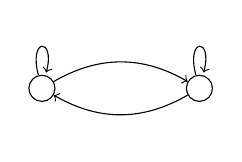
\begin{tikzpicture}
            \graphbox{}{0mm}{0mm}{32mm}{28mm}{-10mm}{-14mm}{
                \node[draw,circle] (1) at (0,0) {};
                \node[draw,circle] (2) at (2,0) {};
                \draw[->] (1) edge[loop above] node[midway, above] { } (1) ;
                % \draw[->] (1) edge[loop below] node[midway, below] {} (1) ;
                \draw[->] (2) edge[loop above] node[midway, above] { } (2) ;
                \draw[->] (1) edge[bend left] node[midway, above] {}  (2)  ;
                \draw[->] (2) edge[bend left] node[midway, below] {} (1)   ;
            }
        \end{tikzpicture}
        \caption{A category with two objects and the recheability as the morphisms}
        \label{fig:preliminaries:category}
    \end{figure}
\end{example}

% cat notation * 
\begin{notation}
    The composition of morphisms \( f : X \to Y \) and \( g : Y \to Z \) is written in diagrammatic order as \( f \star g \), rather than in functional order \( g \circ f \) as is common in litterature. The advantage is that, when reading from left to right, the morphisms appear in the same order as in the corresponding diagram, making the reasoning accompanying diagrams more intuitive. 
\end{notation}  

\begin{definition}[Monomorphism \cite{pierce1991basic,barr1990category}]
    \label{def:cat:homo}
    A morphism \( f : X \to Y \) is \textbf{monic} (or a \textbf{monomorphism}) if for all morphisms \( g \) and \( h \), if \( g \star f = h \star f \), then \( g = h \). A monomorphism is denoted by \( f : X \rightarrowtail Y \). The set of monomorphisms from $X$ to $Y$ is denoted $\opn{Mono}(X,Y)$.
\end{definition} 

\begin{example} 
    Finite edge-labeled directed multigraphs and their homomorphisms form a category, hereafter denoted \textbf{Graph}. Its objects are labeled graphs, its morphisms are graph homomorphisms, and the monomorphisms are injective homomorphisms.
\end{example}

% \begin{definition}[Span \cite{lowe2010graph}]
%     A pair \( (\alpha : A \to B,~\beta : A \to C) \) of morphisms with a common domain is called a \textbf{span}, denoted by \( B \overset{\alpha}{\leftarrow} A \overset{\beta}{\rightarrow} C \).
% \end{definition}
 
% \begin{definition}[Cospan]
%     A pair \( (\beta' : B \to D,~\alpha' : C \to D) \) of morphisms with a common codomain is called a \textbf{cospan}, denoted by \( B \overset{\beta'}{\rightarrow} D \overset{\alpha'}{\leftarrow} C \). 
% \end{definition} 

In category theory, an ordered pair \((\alpha : A \to B,\, \beta : A \to C)\) of morphisms with a common domain is called a \textbf{span} \cite{lowe2010graph}, denoted by
\(
B \overset{\alpha}{\leftarrow} A \overset{\beta}{\rightarrow} C
\). 
% An example of a span $(\alpha, \beta)$ is shown below.
Likewise, an ordered pair \((\beta' : B \to D,\, \alpha' : C \to D)\) of morphisms with a common codomain is called a \textbf{cospan}, denoted by
\(
B \overset{\beta'}{\rightarrow} D \overset{\alpha'}{\leftarrow} C
\). 
% An example of a cospan $(\beta', \alpha')$ is shown below.
A span and a cospan are illustrated in~\autoref{fig:preliminaries:span_cospan}.
\begin{figure}
   \centering
        \resizebox{0.7\textwidth}{!}{
        \begin{tikzpicture} 
            \graphbox{\( L \)}{40mm}{20mm}{34mm}{12mm}{2mm}{2mm}{
                \coordinate (o) at (0mm,-8mm); 
                \node[draw,circle] (l1) at ($(o)+(-10mm,0mm)$) {1};
                \node[draw,circle] (l2) at ($(l1)+(2,0)$) {2};
                \node[draw,circle,red] (l3) at ($(l1) + (1,0)$) {3};
                \draw[->,red] (l1) -- (l3) node[midway,above] {a};
                \draw[->,red] (l3) -- (l2) node[midway,above] {a};
            } 
    
            \graphbox{\( K \)}{0mm}{0mm}{34mm}{12mm}{2mm}{2mm}{
                \coordinate (o) at (0mm,-8mm); 
                \node[draw,circle] (l1) at ($(o)+(-10mm,0mm)$) {1};
                \node[draw,circle] (l2) at ($(l1)+(2,0)$) {2};
            }  
            \graphbox{\(G = L \cup C \)}{90mm}{5mm}{34mm}{27mm}{2mm}{-3mm}{
                \coordinate (o) at (0mm,-8mm); 
                \node[draw,circle] (l1) at ($(o)+(-10mm,0mm)$) {1};
                \node[draw,circle] (l2) at ($(l1)+(2,0)$) {2};
                \node[draw,circle,red] (l3) at ($(l1) + (1,0)$) {3};
                \node[draw,circle,blue] (l4) at ($(l2) + (0,-1)$) {6};
                \draw[->,red] (l1) -- (l3) node[midway,above] {a};
                \draw[->,red] (l3) -- (l2) node[midway,above] {a};
                \draw[->,blue] (l2) -- (l4) node[midway,right] {a};
                \node[draw,circle,blue] (l6) at ($(l1) + (0,-1)$) {7};
                \draw[<-,blue] (l1) -- (l6) node[midway,left] {a};
                \draw[->,blue] (l2) edge[out=-135,in=-45]node[midway,below] {a} (l1) ;
            }   
     
            \graphbox{\( C \)}{40mm}{-20mm}{34mm}{27mm}{2mm}{-3mm}{
                \coordinate (o) at (0mm,-8mm); 
                \node[draw,circle] (l1) at ($(o)+(-10mm,0mm)$) {1};
                \node[draw,circle] (l2) at ($(l1)+(2,0)$) {2};
                \node[draw,circle,blue] (l4) at ($(l2) + (0,-1)$) {6};
                \draw[->,blue] (l2) -- (l4) node[midway,right] {a};
                \draw[->,blue] (l2) edge[out=-135,in=-45]node[midway,below] {a} (l1) ;
                \node[ draw,circle,blue] (l6) at ($(l1) + (0,-1)$) {7};
                \draw[<-,blue] (l1) -- (l6) node[midway,left] {a};
            }      
            % K to L
            \draw[>->] (17mm,5mm) -- node[above] {$\alpha$} (37mm,15mm);
            % C to G
            \draw[>->] (76mm,-28mm)-- node[below] {$\alpha'$} (104mm,-24mm) ;
            % K to C
            \draw[>->] (17mm,-17mm) -- node[below] {$\beta$} (37mm,-28mm);
            % L to G
            \draw[>->] (76mm,16mm) -- node[above] {$\beta'$} (104mm,7mm);
            % \node () at (57mm,-6mm) {$PO$};
        \end{tikzpicture}
        }
        \caption{Span and Cospan}
        \label{fig:preliminaries:span_cospan}
\end{figure}

\begin{definition}[Diagram \cite{barr1990category}]
    \label{def:cat:diagram}
    Let \( G \) be an unlabeled graph. A \textbf{diagram} (in \( \mathcal{C} \) of shape \( G \)) is a homomorphism of unlabeled graphs \( h : G \to C \) where \( C \) is the underlying unlabeled graph of the category \( \mathcal{C} \). A diagram is \textbf{commutative} if, for all nodes \( u \), \( v \), and any two paths from \( u \) to \( v \) in the unlabeled graph \( G \):

    \begin{center}
    \resizebox{12cm}{!}{
        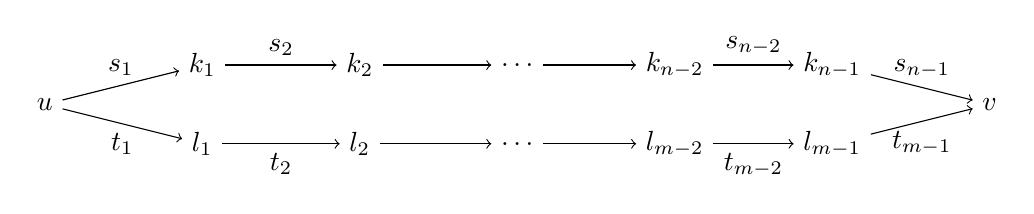
\begin{tikzpicture}
        \node (u) at (0,0) {\( u \)};
        \node (k1) at (2,0.5) {\( k_1 \)};
        \node (k2) at (4,0.5) {\( k_2 \)};
        \node (ketc) at (6,0.5) {\( \dots \)};
        \node (knm2) at (8,0.5) {\( k_{n-2} \)};
        \node (knm1) at (10,0.5) {\( k_{n-1} \)};
        \node (v) at (12,0) {\( v \)};
        \node (l1) at (2,-0.5) {\( l_1 \)};
        \node (l2) at (4,-0.5) {\( l_2 \)};
        \node (letc) at (6,-0.5) {\( \dots \)};
        \node (lnm2) at (8,-0.5) {\( l_{m-2} \)};
        \node (lnm1) at (10,-0.5) {\( l_{m-1} \)};
        \draw[->] (u) -- (k1) node [midway,above] {\( s_1 \)};
        \draw[->] (k1) -- (k2) node [midway,above] {\( s_2 \)};
        \draw[->] (k2) -- (ketc);
        \draw[->] (ketc) -- (knm2); 
        \draw[->] (knm2) -- (knm1) node[midway,above] {\( s_{n-2} \)}; 
        \draw[->] (knm1) -- (v) node[midway,above] {\( s_{n-1} \)}; 
        \draw[->] (u) -- (l1) node[midway,below] {\( t_1 \)};
        \draw[->] (l1) -- (l2) node[midway,below] {\( t_2 \)};
        \draw[->] (l2) -- (letc);
        \draw[->] (letc) -- (lnm2); 
        \draw[->] (lnm2) -- (lnm1) node[midway,below] {\( t_{m-2} \)}; 
        \draw[->] (lnm1) -- (v) node[midway,below] {\( t_{m-1} \)}; 
        \end{tikzpicture}
    }
    \end{center}
    \noindent
    the equality \( h(s_1) \star h(s_2) \star \dots  \star h(s_{n-1}) = h(t_1) \star h(t_2) \star \dots  \star h(t_{m-1}) \) holds.
\end{definition}

\begin{example}
    A commutative diagram in the category \textbf{Graph} of edge-labeled directed multigraphs is illustrated in~\autoref{fig:preliminaries:commutative_diagram}. The symbol $\mathop{=}$ in the center of the diagram
    is used to indicate that the two paths from node 1 to node 2 are equal.
 
    \begin{figure}
        \centering
        \resizebox{0.7\textwidth}{!}{
        \begin{tikzpicture} 
            \graphbox{\( L \)}{40mm}{20mm}{34mm}{12mm}{2mm}{2mm}{
                \coordinate (o) at (0mm,-8mm); 
                \node[draw,circle] (l1) at ($(o)+(-10mm,0mm)$) {1};
                \node[draw,circle] (l2) at ($(l1)+(2,0)$) {2};
                \node[draw,circle,red] (l3) at ($(l1) + (1,0)$) {3};
                \draw[->,red] (l1) -- (l3) node[midway,above] {a};
                \draw[->,red] (l3) -- (l2) node[midway,above] {a};
            } 
    
            \graphbox{\( K \)}{0mm}{0mm}{34mm}{12mm}{2mm}{2mm}{
                \coordinate (o) at (0mm,-8mm); 
                \node[draw,circle] (l1) at ($(o)+(-10mm,0mm)$) {1};
                \node[draw,circle] (l2) at ($(l1)+(2,0)$) {2};
            }  
            \graphbox{\(G = L \cup C \)}{90mm}{5mm}{34mm}{27mm}{2mm}{-3mm}{
                \coordinate (o) at (0mm,-8mm); 
                \node[draw,circle] (l1) at ($(o)+(-10mm,0mm)$) {1};
                \node[draw,circle] (l2) at ($(l1)+(2,0)$) {2};
                \node[draw,circle,red] (l3) at ($(l1) + (1,0)$) {3};
                \node[draw,circle,blue] (l4) at ($(l2) + (0,-1)$) {6};
                \draw[->,red] (l1) -- (l3) node[midway,above] {a};
                \draw[->,red] (l3) -- (l2) node[midway,above] {a};
                \draw[->,blue] (l2) -- (l4) node[midway,right] {a};
                \node[draw,circle,blue] (l6) at ($(l1) + (0,-1)$) {7};
                \draw[<-,blue] (l1) -- (l6) node[midway,left] {a};
                \draw[->,blue] (l2) edge[out=-135,in=-45]node[midway,below] {a} (l1) ;
            }   
     
            \graphbox{\( C \)}{40mm}{-20mm}{34mm}{27mm}{2mm}{-3mm}{
                \coordinate (o) at (0mm,-8mm); 
                \node[draw,circle] (l1) at ($(o)+(-10mm,0mm)$) {1};
                \node[draw,circle] (l2) at ($(l1)+(2,0)$) {2};
                \node[draw,circle,blue] (l4) at ($(l2) + (0,-1)$) {6};
                \draw[->,blue] (l2) -- (l4) node[midway,right] {a};
                \draw[->,blue] (l2) edge[out=-135,in=-45]node[midway,below] {a} (l1) ;
                \node[ draw,circle,blue] (l6) at ($(l1) + (0,-1)$) {7};
                \draw[<-,blue] (l1) -- (l6) node[midway,left] {a};
            }      
            % K to L
            \draw[>->] (17mm,5mm) -- node[above] {$\alpha$} (37mm,15mm);
            % C to G
            \draw[>->] (76mm,-28mm)-- node[below] {$\alpha'$} (104mm,-24mm) ;
            % K to C
            \draw[>->] (17mm,-17mm) -- node[below] {$\beta$} (37mm,-28mm);
            % L to G
            \draw[>->] (76mm,16mm) -- node[above] {$\beta'$} (104mm,7mm);
            \node () at (57mm,-6mm) {$\mathop{=}$};
        \end{tikzpicture}
        }
        \caption{A commutative diagram}
        \label{fig:preliminaries:commutative_diagram}
    \end{figure}
\end{example}
The pushout is a construction in category theory that can often be thought of as the construction of a new structure from two given structures by gluing them along a common interface structure.
\begin{definition}[Pushout \cite{barr1990category}]
    \label{def:cat:po}
    \ \newline
\noindent
\begin{minipage}{0.7\textwidth}  
    A \textbf{pushout} of a span \( B \overset{\alpha}{\leftarrow} A \overset{\beta}{\rightarrow} C \), as shown on the right, is defined as a cospan \( B \overset{\beta'}{\rightarrow} D \overset{\alpha'}{\leftarrow} C \) such that \( \alpha \star \beta' = \beta \star \alpha' \), and for every cospan \( B \overset{\gamma'}{\rightarrow} E \overset{\gamma}{\leftarrow} C \), if \( \alpha \star \gamma' = \beta \star \gamma \) holds, then there exists a unique morphism \(\delta : D \to E\) such that \( \gamma' = \beta' \star \delta \) and \( \gamma = \alpha' \star \delta \).
\end{minipage}
\hfill
\begin{minipage}{0.299\textwidth}
    \hfill
\resizebox{0.9\textwidth}{!}{
           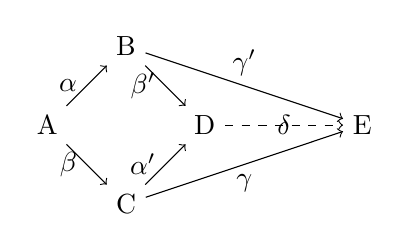
\begin{tikzpicture}
                \node (i) at (0,0) {A};
                \node (r) at (1,1) {B};
                \node (c) at (1,-1) {C};
                \node (h) at (2,0) {D};
                % \node () at (1,-1) {\( \Delta \)};
                \draw[->]  (i) -- (r) node [midway,left] {$ \alpha $};
                \draw[->] (c) -- (h) node [midway,left] {$ \alpha' $};
                \draw[->] (r) -- (h) node[midway, left] {$ \beta' $};
                \draw[->] (i) -- (c) node[midway, left] {$ \beta $};
                \node (d') at (4,0) {E};
                \draw[->] (c) -- (d') node [midway,below]{$ \gamma $};
                \draw[->] (r) -- (d') node [midway,above]{$ \gamma' $};
                \draw[->,dashed] (h) -- (d') node [midway]{$ \delta $};
            \end{tikzpicture}
}
\end{minipage}
The diagram involving \( (\alpha, \beta, \alpha', \beta') \) is called the \textbf{pushout square}, with \(D\) as the \textbf{pushout object}. The existence of a unique morphism is known as the \textbf{universal mapping property of the pushout}.
\end{definition} 

\begin{example}
    The diagram in~\autoref{fig:preliminaries:pushout_injective} is a pushout square in the category \textbf{Graph} of edge-labeled directed multigraphs. In this example, both $\alpha$ and $\beta$ are injective morphisms. Therefore, the pushout object $G$ can be constructed easily by taking the interface graph $K$ and adding elements from $L$ and $C$ which are not present in $K$.
    \begin{figure}[hbtp]
        \centering
        \resizebox{0.7\textwidth}{!}{
        \begin{tikzpicture} 
            \graphbox{\( L \)}{40mm}{20mm}{34mm}{12mm}{2mm}{2mm}{
                \coordinate (o) at (0mm,-8mm); 
                \node[draw,circle] (l1) at ($(o)+(-10mm,0mm)$) {1};
                \node[draw,circle] (l2) at ($(l1)+(2,0)$) {2};
                \node[draw,circle,red] (l3) at ($(l1) + (1,0)$) {3};
                \draw[->,red] (l1) -- (l3) node[midway,above] {a};
                \draw[->,red] (l3) -- (l2) node[midway,above] {a};
            } 
    
            \graphbox{\( K \)}{0mm}{0mm}{34mm}{12mm}{2mm}{2mm}{
                \coordinate (o) at (0mm,-8mm); 
                \node[draw,circle] (l1) at ($(o)+(-10mm,0mm)$) {1};
                \node[draw,circle] (l2) at ($(l1)+(2,0)$) {2};
            }  
            \graphbox{\(G  \)}{90mm}{5mm}{34mm}{27mm}{2mm}{-3mm}{
                \coordinate (o) at (0mm,-8mm); 
                \node[draw,circle] (l1) at ($(o)+(-10mm,0mm)$) {1};
                \node[draw,circle] (l2) at ($(l1)+(2,0)$) {2};
                \node[draw,circle,red] (l3) at ($(l1) + (1,0)$) {3};
                \node[draw,circle,blue] (l4) at ($(l2) + (0,-1)$) {6};
                \draw[->,red] (l1) -- (l3) node[midway,above] {a};
                \draw[->,red] (l3) -- (l2) node[midway,above] {a};
                \draw[->,blue] (l2) -- (l4) node[midway,right] {a};
                \node[draw,circle,blue] (l6) at ($(l1) + (0,-1)$) {7};
                \draw[<-,blue] (l1) -- (l6) node[midway,left] {a};
                \draw[->,blue] (l2) edge[out=-135,in=-45]node[midway,below] {a} (l1) ;
            }   
     
            \graphbox{\( C \)}{40mm}{-20mm}{34mm}{27mm}{2mm}{-3mm}{
                \coordinate (o) at (0mm,-8mm); 
                \node[draw,circle] (l1) at ($(o)+(-10mm,0mm)$) {1};
                \node[draw,circle] (l2) at ($(l1)+(2,0)$) {2};
                \node[draw,circle,blue] (l4) at ($(l2) + (0,-1)$) {6};
                \draw[->,blue] (l2) -- (l4) node[midway,right] {a};
                \draw[->,blue] (l2) edge[out=-135,in=-45]node[midway,below] {a} (l1) ;
                \node[ draw,circle,blue] (l6) at ($(l1) + (0,-1)$) {7};
                \draw[<-,blue] (l1) -- (l6) node[midway,left] {a};
            }      
            % K to L
            \draw[>->] (17mm,5mm) -- node[above] {$\alpha$} (37mm,15mm);
            % C to G
            \draw[>->] (76mm,-28mm)-- node[below] {$\alpha'$} (104mm,-24mm) ;
            % K to C
            \draw[>->] (17mm,-17mm) -- node[below] {$\beta$} (37mm,-28mm);
            % L to G
            \draw[>->] (76mm,16mm) -- node[above] {$\beta'$} (104mm,7mm);
            \node () at (57mm,-6mm) {$PO$};
        \end{tikzpicture}
        }
        \caption{A pushout square with injective morphisms}
        \label{fig:preliminaries:pushout_injective}
    \end{figure}
\end{example}

\begin{example}
    The diagram in~\autoref{fig:preliminaries:pushout_non_injective} is a pushout square in the category \textbf{Graph} of edge-labeled directed multigraphs. In this example, $\beta$ is not injective. Therefore, some elements are merged in the pushout object $G$.

    \begin{figure}[hbtp]
        \centering 
        \resizebox{0.7\textwidth}{!}{
        \begin{tikzpicture} 
            \graphbox{\( L \)}{40mm}{20mm}{34mm}{20mm}{2mm}{2mm}{
                \coordinate (o) at (0mm,-8mm); 
                \node[draw,circle] (l1) at ($(o)+(-10mm,0mm)$) {1};
                \node[draw,circle] (l2) at ($(l1)+(2,0)$) {2};
                \draw[->,red] (l2) edge[out=-135,in=-45]node[midway,below] {a} (l1) ;
                \node[draw,circle,red] (l3) at ($(l1) + (1,0)$) {3};
                \draw[->,red] (l1) -- (l3) node[midway,above] {a};
                \draw[->,red] (l3) -- (l2) node[midway,above] {a};
            } 
    
            \graphbox{\( K \)}{0mm}{0mm}{34mm}{12mm}{2mm}{2mm}{
                \coordinate (o) at (0mm,-8mm); 
                \node[draw,circle] (l1) at ($(o)+(-10mm,0mm)$) {1};
                \node[draw,circle] (l2) at ($(l1)+(2,0)$) {2};
            }  
            \graphbox{\(G  \)}{110mm}{5mm}{34mm}{40mm}{2mm}{-3mm}{
                \coordinate (o) at (0mm,-20mm); 
                 \node[draw,circle] (l1) at ($(o)+(0,0)$) {1\ 2};
                % \node[draw,circle] (l1) at ($(o)+(-10mm,0mm)$) {1};
                % \node[draw,circle] (l2) at ($(l1)+(2,0)$) {2};
                \draw[->,red] (l1) edge[loop below] node[midway, below] {$a$} (l1) ;
                \node[draw,circle,red] (l3) at ($(l1) + (0,1.4)$) {3};
                \node[draw,circle,blue] (l4) at ($(l1) + (1,-1)$) {6};
                \draw[->,red] (l1) edge[bend left] node[midway,left] {a} (l3);
                \draw[->,red] (l3) edge[bend left] node[midway,right] {a} (l1);
                \draw[->,blue] (l1) edge  node[midway,right] {a} (l4);
                \node[draw,circle,blue] (l6) at ($(l1) + (-1,-1)$) {7};
                \draw[<-,blue] (l1) edge node[midway,left] {a} (l6) ;
                % \draw[->,blue] (l1) edge[out=-135,in=-45]node[midway,below] {a} (l1) ;
            }   
     
            \graphbox{\( C \)}{40mm}{-20mm}{34mm}{35mm}{2mm}{-3mm}{
                \coordinate (o) at (0mm,-14mm); 
                \node[draw,circle] (l1) at ($(o)+(0,0)$) {1\ 2};
                % \node[draw,circle] (l2) at ($(l1)+(2,0)$) {2};
                \node[draw,circle,blue] (l4) at ($(l1) + (1,-1)$) {6};
                \draw[->,blue] (l1) -- (l4) node[midway,right] {a};
                % \draw[->,blue] (l1) edge[loop above] node[midway, above] {a} (l1) ;
                \node[ draw,circle,blue] (l6) at ($(l1) + (-1,-1)$) {7};
                \draw[<-,blue] (l1) -- (l6) node[midway,left] {a};
            }
            % K to L  
            \draw[>->] (17mm,5mm) -- node[above] {$\alpha$} (37mm,15mm);
            % C to G
            \draw[>->] (76mm,-28mm)-- node[below] {$\alpha'$} (104mm,-24mm) ;
            % K to C
            \draw[->] (17mm,-17mm) -- node[below] {$\beta$} (37mm,-28mm);
            % L to G
            \draw[->] (76mm,16mm) -- node[above] {$\beta'$} (104mm,7mm);
            \node () at (57mm,-6mm) {$PO$};
        \end{tikzpicture}
        }
        \caption{A pushout square with a non-injective morphism}
        \label{fig:preliminaries:pushout_non_injective}
    \end{figure} 
\end{example}
The pullback is the dual construction of the pushout in category theory, and it can be thought of as construction of the interface structure along which two structures are glued together. (to double check)
\begin{definition}[Pullback \cite{pierce1991basic}]
    \label{def:cat:pb}
    \ \newline
\noindent
\begin{minipage}{0.7\textwidth}  
   A \textbf{pullback} of a cospan \(B \overset{\beta'}{\rightarrow} D \overset{\alpha'}{\leftarrow} C \), as shown on the right, is defined as a span \( B \overset{\alpha}{\leftarrow} A \overset{\beta}{\rightarrow} C \) such that \( \alpha \star \beta' = \beta \star \alpha' \), and for every span \( B \overset{\gamma'}{\leftarrow} E \overset{\gamma}{\rightarrow} C \) if \(\gamma' \star \beta' = \gamma \star \alpha'\) holds, then there exists a unique morphism \(\delta: E \to A\) such that $\gamma' = \delta \star \alpha$ and $\gamma = \delta \star \beta$. 
\end{minipage}
\hfill
\begin{minipage}{0.299\textwidth}
    \hfill
\resizebox{0.9\textwidth}{!}{
            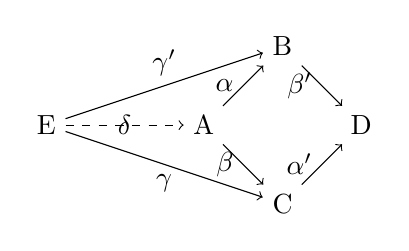
\begin{tikzpicture}
                \node (i) at (0,0) {A};
                \node (r) at (1,1) {B};
                \node (c) at (1,-1) {C};
                \node (h) at (2,0) {D};
                % \node () at (1,-1) {\( \Delta \)};
                \draw[->]  (i) -- (r) node [midway,left] {$\alpha$};
                \draw[->] (c) -- (h) node [midway,left] {$\alpha'$};
                \draw[->] (r) -- (h) node[midway, left] {$\beta'$};
                \draw[->] (i) -- (c) node[midway, left] {$\beta$};
                \node (d') at (-2,0) {E};
                \draw[<-] (c) -- (d') node [midway,below]{$\gamma$};
                \draw[<-] (r) -- (d') node [midway,above]{$\gamma'$};
                \draw[->, dashed] (d') -- (i) node [midway]{$\delta$};
            \end{tikzpicture}
}
\end{minipage}
The diagram involving \( (\alpha, \beta, \alpha', \beta') \) is called the \textbf{pullback square}, with \(A\) as the \textbf{pullback object}. The existence of a unique morphism is known as the \textbf{universal mapping property of the pullback}.
\end{definition} 


\begin{example}
    The following diagram is a pullback square in the category \textbf{Graph} of edge-labeled directed multigraphs. 
    \begin{center}  
        \resizebox{0.7\textwidth}{!}{
        \begin{tikzpicture} 
            \graphbox{\( L \)}{40mm}{20mm}{34mm}{20mm}{2mm}{2mm}{
                \coordinate (o) at (0mm,-8mm); 
                \node[draw,circle] (l1) at ($(o)+(-10mm,0mm)$) {1};
                \node[draw,circle] (l2) at ($(l1)+(2,0)$) {2};
                \draw[->,red] (l2) edge[out=-135,in=-45]node[midway,below] {a} (l1) ;
                \node[draw,circle,red] (l3) at ($(l1) + (1,0)$) {3};
                \draw[->,red] (l1) -- (l3) node[midway,above] {a};
                \draw[->,red] (l3) -- (l2) node[midway,above] {a};
            } 
    
            \graphbox{\( K \)}{0mm}{0mm}{34mm}{12mm}{2mm}{2mm}{
                \coordinate (o) at (0mm,-8mm); 
                \node[draw,circle] (l1) at ($(o)+(-10mm,0mm)$) {1};
                \node[draw,circle] (l2) at ($(l1)+(2,0)$) {2};
            }  
            \graphbox{\(G  \)}{110mm}{5mm}{34mm}{40mm}{2mm}{-3mm}{
                \coordinate (o) at (0mm,-20mm); 
                 \node[draw,circle] (l1) at ($(o)+(0,0)$) {1\ 2};
                % \node[draw,circle] (l1) at ($(o)+(-10mm,0mm)$) {1};
                % \node[draw,circle] (l2) at ($(l1)+(2,0)$) {2};
                \draw[->,red] (l1) edge[loop below] node[midway, below] {$a$} (l1) ;
                \node[draw,circle,red] (l3) at ($(l1) + (0,1.4)$) {3};
                \node[draw,circle,blue] (l4) at ($(l1) + (1,-1)$) {6};
                \draw[->,red] (l1) edge[bend left] node[midway,left] {a} (l3);
                \draw[->,red] (l3) edge[bend left] node[midway,right] {a} (l1);
                \draw[->,blue] (l1) edge  node[midway,right] {a} (l4);
                \node[draw,circle,blue] (l6) at ($(l1) + (-1,-1)$) {7};
                \draw[<-,blue] (l1) edge node[midway,left] {a} (l6) ;
                % \draw[->,blue] (l1) edge[out=-135,in=-45]node[midway,below] {a} (l1) ;
            }   
     
            \graphbox{\( C \)}{40mm}{-20mm}{34mm}{35mm}{2mm}{-3mm}{
                \coordinate (o) at (0mm,-14mm); 
                \node[draw,circle] (l1) at ($(o)+(0,0)$) {1\ 2};
                % \node[draw,circle] (l2) at ($(l1)+(2,0)$) {2};
                \node[draw,circle,blue] (l4) at ($(l1) + (1,-1)$) {6};
                \draw[->,blue] (l1) -- (l4) node[midway,right] {a};
                % \draw[->,blue] (l1) edge[loop above] node[midway, above] {a} (l1) ;
                \node[ draw,circle,blue] (l6) at ($(l1) + (-1,-1)$) {7};
                \draw[<-,blue] (l1) -- (l6) node[midway,left] {a};
            }
            % K to L  
            \draw[>->] (17mm,5mm) -- node[above] {$\alpha$} (37mm,15mm);
            % C to G
            \draw[>->] (76mm,-28mm)-- node[below] {$\alpha'$} (104mm,-24mm) ;
            % K to C
            \draw[->] (17mm,-17mm) -- node[below] {$\beta$} (37mm,-28mm);
            % L to G
            \draw[->] (76mm,16mm) -- node[above] {$\beta'$} (104mm,7mm);
            \node () at (57mm,-6mm) {$PB$};
        \end{tikzpicture}
        }
    \end{center} 
    In fact, there are three possible spans \( B \overset{\gamma'}{\leftarrow} E \overset{\gamma}{\rightarrow} C \) such that \(\gamma' \star \beta' = \gamma \star \alpha'\) holds, and for each of them, there exists a unique morphism \(\delta: E \to A\) such that $\gamma' = \delta \star \alpha$ and $\gamma = \delta \star \beta$, as shown in the following three diagrams:

    \begin{center}  
        \resizebox{0.9\textwidth}{!}{
        \begin{tikzpicture} 
            \graphbox{\( E_1 \)}{-50mm}{0mm}{34mm}{12mm}{2mm}{2mm}{
                \coordinate (o) at (0mm,-8mm); 
                \node[draw,circle] (l1) at ($(o)+(-10mm,0mm)$) {1};
                \node[draw,circle] (l2) at ($(l1)+(2,0)$) {2};
            }  
            \graphbox{\( L \)}{40mm}{20mm}{34mm}{20mm}{2mm}{2mm}{
                \coordinate (o) at (0mm,-8mm); 
                \node[draw,circle] (l1) at ($(o)+(-10mm,0mm)$) {1};
                \node[draw,circle] (l2) at ($(l1)+(2,0)$) {2};
                \draw[->,red] (l2) edge[out=-135,in=-45]node[midway,below] {a} (l1) ;
                \node[draw,circle,red] (l3) at ($(l1) + (1,0)$) {3};
                \draw[->,red] (l1) -- (l3) node[midway,above] {a};
                \draw[->,red] (l3) -- (l2) node[midway,above] {a};
            } 
    
            \graphbox{\( K \)}{0mm}{0mm}{34mm}{12mm}{2mm}{2mm}{
                \coordinate (o) at (0mm,-8mm); 
                \node[draw,circle] (l1) at ($(o)+(-10mm,0mm)$) {1};
                \node[draw,circle] (l2) at ($(l1)+(2,0)$) {2};
            }  

             \graphbox{\( C \)}{40mm}{-20mm}{34mm}{35mm}{2mm}{-3mm}{
                \coordinate (o) at (0mm,-14mm); 
                \node[draw,circle] (l1) at ($(o)+(0,0)$) {1\ 2};
                % \node[draw,circle] (l2) at ($(l1)+(2,0)$) {2};
                \node[draw,circle,blue] (l4) at ($(l1) + (1,-1)$) {6};
                \draw[->,blue] (l1) -- (l4) node[midway,right] {a};
                % \draw[->,blue] (l1) edge[loop above] node[midway, above] {a} (l1) ;
                \node[ draw,circle,blue] (l6) at ($(l1) + (-1,-1)$) {7};
                \draw[<-,blue] (l1) -- (l6) node[midway,left] {a};
            }

            \graphbox{\(G  \)}{110mm}{5mm}{34mm}{40mm}{2mm}{-3mm}{
                \coordinate (o) at (0mm,-20mm); 
                 \node[draw,circle] (l1) at ($(o)+(0,0)$) {1\ 2};
                % \node[draw,circle] (l1) at ($(o)+(-10mm,0mm)$) {1};
                % \node[draw,circle] (l2) at ($(l1)+(2,0)$) {2};
                \draw[->,red] (l1) edge[loop below] node[midway, below] {$a$} (l1) ;
                \node[draw,circle,red] (l3) at ($(l1) + (0,1.4)$) {3};
                \node[draw,circle,blue] (l4) at ($(l1) + (1,-1)$) {6};
                \draw[->,red] (l1) edge[bend left] node[midway,left] {a} (l3);
                \draw[->,red] (l3) edge[bend left] node[midway,right] {a} (l1);
                \draw[->,blue] (l1) edge  node[midway,right] {a} (l4);
                \node[draw,circle,blue] (l6) at ($(l1) + (-1,-1)$) {7};
                \draw[<-,blue] (l1) edge node[midway,left] {a} (l6) ;
                % \draw[->,blue] (l1) edge[out=-135,in=-45]node[midway,below] {a} (l1) ;
            }   
            % E to K
            \draw[>->] (-15mm,-6mm) -- node[above] {$\delta_1$} (-1mm,-6mm);
            % E to L
            \draw[>->] (-33mm,5mm) -- node[above] {$\gamma'_1$} (33mm,15mm);
            % K to L  
            \draw[>->] (17mm,5mm) -- node[above] {$\alpha$} (37mm,15mm);
            % C to G
            \draw[>->] (76mm,-28mm)-- node[below] {$\alpha'$} (104mm,-24mm) ;
            % K to C
            \draw[->] (17mm,-17mm) -- node[below] {$\beta$} (37mm,-28mm);
             % E to C
            \draw[->] (-33mm,-17mm) -- node[below] {$\gamma_1$} (33mm,-28mm);
            % L to G
            \draw[->] (76mm,16mm) -- node[above] {$\beta'$} (104mm,7mm);
            % \node () at (57mm,-6mm) {$PB$};
        \end{tikzpicture}
        }
    \end{center} 

    \begin{center}  
        \resizebox{0.9\textwidth}{!}{
        \begin{tikzpicture} 
            \graphbox{\( E_2 \)}{-50mm}{0mm}{34mm}{12mm}{2mm}{2mm}{
                \coordinate (o) at (0mm,-8mm); 
                \node[draw,circle] (l1) at ($(o)+(-10mm,0mm)$) {1};
                % \node[draw,circle] (l2) at ($(l1)+(2,0)$) {2};
            }  
            \graphbox{\( L \)}{40mm}{20mm}{34mm}{20mm}{2mm}{2mm}{
                \coordinate (o) at (0mm,-8mm); 
                \node[draw,circle] (l1) at ($(o)+(-10mm,0mm)$) {1};
                \node[draw,circle] (l2) at ($(l1)+(2,0)$) {2};
                \draw[->,red] (l2) edge[out=-135,in=-45]node[midway,below] {a} (l1) ;
                \node[draw,circle,red] (l3) at ($(l1) + (1,0)$) {3};
                \draw[->,red] (l1) -- (l3) node[midway,above] {a};
                \draw[->,red] (l3) -- (l2) node[midway,above] {a};
            } 
    
            \graphbox{\( K \)}{0mm}{0mm}{34mm}{12mm}{2mm}{2mm}{
                \coordinate (o) at (0mm,-8mm); 
                \node[draw,circle] (l1) at ($(o)+(-10mm,0mm)$) {1};
                \node[draw,circle] (l2) at ($(l1)+(2,0)$) {2};
            }  

             \graphbox{\( C \)}{40mm}{-20mm}{34mm}{35mm}{2mm}{-3mm}{
                \coordinate (o) at (0mm,-14mm); 
                \node[draw,circle] (l1) at ($(o)+(0,0)$) {1\ 2};
                % \node[draw,circle] (l2) at ($(l1)+(2,0)$) {2};
                \node[draw,circle,blue] (l4) at ($(l1) + (1,-1)$) {6};
                \draw[->,blue] (l1) -- (l4) node[midway,right] {a};
                % \draw[->,blue] (l1) edge[loop above] node[midway, above] {a} (l1) ;
                \node[ draw,circle,blue] (l6) at ($(l1) + (-1,-1)$) {7};
                \draw[<-,blue] (l1) -- (l6) node[midway,left] {a};
            }

            \graphbox{\(G  \)}{110mm}{5mm}{34mm}{40mm}{2mm}{-3mm}{
                \coordinate (o) at (0mm,-20mm); 
                 \node[draw,circle] (l1) at ($(o)+(0,0)$) {1\ 2};
                % \node[draw,circle] (l1) at ($(o)+(-10mm,0mm)$) {1};
                % \node[draw,circle] (l2) at ($(l1)+(2,0)$) {2};
                \draw[->,red] (l1) edge[loop below] node[midway, below] {$a$} (l1) ;
                \node[draw,circle,red] (l3) at ($(l1) + (0,1.4)$) {3};
                \node[draw,circle,blue] (l4) at ($(l1) + (1,-1)$) {6};
                \draw[->,red] (l1) edge[bend left] node[midway,left] {a} (l3);
                \draw[->,red] (l3) edge[bend left] node[midway,right] {a} (l1);
                \draw[->,blue] (l1) edge  node[midway,right] {a} (l4);
                \node[draw,circle,blue] (l6) at ($(l1) + (-1,-1)$) {7};
                \draw[<-,blue] (l1) edge node[midway,left] {a} (l6) ;
                % \draw[->,blue] (l1) edge[out=-135,in=-45]node[midway,below] {a} (l1) ;
            }   
            % E to K
            \draw[>->] (-15mm,-6mm) -- node[above] {$\delta_2$} (-1mm,-6mm);
            % E to L
            \draw[>->] (-33mm,5mm) -- node[above] {$\gamma'_2$} (33mm,15mm);
            % K to L  
            \draw[>->] (17mm,5mm) -- node[above] {$\alpha$} (37mm,15mm);
            % C to G
            \draw[>->] (76mm,-28mm)-- node[below] {$\alpha'$} (104mm,-24mm) ;
            % K to C
            \draw[->] (17mm,-17mm) -- node[below] {$\beta$} (37mm,-28mm);
            % E to C
            \draw[->] (-33mm,-17mm) -- node[below] {$\gamma_2$} (33mm,-28mm);
            % L to G
            \draw[->] (76mm,16mm) -- node[above] {$\beta'$} (104mm,7mm);
            % \node () at (57mm,-6mm) {$PB$};
        \end{tikzpicture}
        }
    \end{center} 

    \begin{center}  
        \resizebox{0.9\textwidth}{!}{
        \begin{tikzpicture} 
            \graphbox{\( E_3 \)}{-50mm}{0mm}{34mm}{12mm}{2mm}{2mm}{
                \coordinate (o) at (0mm,-8mm); 
                % \node[draw,circle] (l1) at ($(o)+(-10mm,0mm)$) {1};
                \node[draw,circle] (l2) at ($(o)+(10mm,0mm)$) {2};
            }  
            \graphbox{\( L \)}{40mm}{20mm}{34mm}{20mm}{2mm}{2mm}{
                \coordinate (o) at (0mm,-8mm); 
                \node[draw,circle] (l1) at ($(o)+(-10mm,0mm)$) {1};
                \node[draw,circle] (l2) at ($(l1)+(2,0)$) {2};
                \draw[->,red] (l2) edge[out=-135,in=-45]node[midway,below] {a} (l1) ;
                \node[draw,circle,red] (l3) at ($(l1) + (1,0)$) {3};
                \draw[->,red] (l1) -- (l3) node[midway,above] {a};
                \draw[->,red] (l3) -- (l2) node[midway,above] {a};
            } 
    
            \graphbox{\( K \)}{0mm}{0mm}{34mm}{12mm}{2mm}{2mm}{
                \coordinate (o) at (0mm,-8mm); 
                \node[draw,circle] (l1) at ($(o)+(-10mm,0mm)$) {1};
                \node[draw,circle] (l2) at ($(l1)+(2,0)$) {2};
            }  

             \graphbox{\( C \)}{40mm}{-20mm}{34mm}{35mm}{2mm}{-3mm}{
                \coordinate (o) at (0mm,-14mm); 
                \node[draw,circle] (l1) at ($(o)+(0,0)$) {1\ 2};
                % \node[draw,circle] (l2) at ($(l1)+(2,0)$) {2};
                \node[draw,circle,blue] (l4) at ($(l1) + (1,-1)$) {6};
                \draw[->,blue] (l1) -- (l4) node[midway,right] {a};
                % \draw[->,blue] (l1) edge[loop above] node[midway, above] {a} (l1) ;
                \node[ draw,circle,blue] (l6) at ($(l1) + (-1,-1)$) {7};
                \draw[<-,blue] (l1) -- (l6) node[midway,left] {a};
            }

            \graphbox{\(G  \)}{110mm}{5mm}{34mm}{40mm}{2mm}{-3mm}{
                \coordinate (o) at (0mm,-20mm); 
                 \node[draw,circle] (l1) at ($(o)+(0,0)$) {1\ 2};
                % \node[draw,circle] (l1) at ($(o)+(-10mm,0mm)$) {1};
                % \node[draw,circle] (l2) at ($(l1)+(2,0)$) {2};
                \draw[->,red] (l1) edge[loop below] node[midway, below] {$a$} (l1) ;
                \node[draw,circle,red] (l3) at ($(l1) + (0,1.4)$) {3};
                \node[draw,circle,blue] (l4) at ($(l1) + (1,-1)$) {6};
                \draw[->,red] (l1) edge[bend left] node[midway,left] {a} (l3);
                \draw[->,red] (l3) edge[bend left] node[midway,right] {a} (l1);
                \draw[->,blue] (l1) edge  node[midway,right] {a} (l4);
                \node[draw,circle,blue] (l6) at ($(l1) + (-1,-1)$) {7};
                \draw[<-,blue] (l1) edge node[midway,left] {a} (l6) ;
                % \draw[->,blue] (l1) edge[out=-135,in=-45]node[midway,below] {a} (l1) ;
            }   
            % E to K
            \draw[>->] (-15mm,-6mm) -- node[above] {$\delta_3$} (-1mm,-6mm);
            % E to L
            \draw[>->] (-33mm,5mm) -- node[above] {$\gamma'_3$} (33mm,15mm);
            % K to L  
            \draw[>->] (17mm,5mm) -- node[above] {$\alpha$} (37mm,15mm);
            % C to G
            \draw[>->] (76mm,-28mm)-- node[below] {$\alpha'$} (104mm,-24mm) ;
            % K to C
            \draw[->] (17mm,-17mm) -- node[below] {$\beta$} (37mm,-28mm);
             % E to C
            \draw[->] (-33mm,-17mm) -- node[below] {$\gamma_3$} (33mm,-28mm);
            % L to G
            \draw[->] (76mm,16mm) -- node[above] {$\beta'$} (104mm,7mm);
            % \node () at (57mm,-6mm) {$=$};
        \end{tikzpicture}
        }
    \end{center} 
\end{example}


\begin{example}
    The following diagram is a pullback square in the category \textbf{Graph} of edge-labeled directed multigraphs.
    \begin{center}  
        \resizebox{0.7\textwidth}{!}{
        \begin{tikzpicture} 
            \graphbox{\( L \)}{40mm}{20mm}{34mm}{20mm}{2mm}{2mm}{
                \coordinate (o) at (0mm,-8mm); 
                \node[draw,circle] (l1) at ($(o)+(-10mm,0mm)$) {1};
                \node[draw,circle] (l2) at ($(l1)+(2,0)$) {2};
                \draw[->,red] (l2) edge[out=-135,in=-45]node[midway,below] {a} (l1) ;
                \node[draw,circle,red] (l3) at ($(l1) + (1,0)$) {3};
                \draw[->,red] (l1) -- (l3) node[midway,above] {a};
                \draw[->,red] (l3) -- (l2) node[midway,above] {a};
            } 
    
            \graphbox{\( K \)}{0mm}{0mm}{34mm}{12mm}{2mm}{2mm}{
                \coordinate (o) at (0mm,-8mm); 
                \node[draw,circle] (l1) at ($(o)+(-10mm,0mm)$) {1};
                \node[draw,circle] (l2) at ($(l1)+(2,0)$) {2};
            }  
            \graphbox{\(G  \)}{110mm}{5mm}{34mm}{40mm}{2mm}{-3mm}{
                \coordinate (o) at (0mm,-20mm); 
                 \node[draw,circle] (l1) at ($(o)+(0,0)$) {1\ 2};
                % \node[draw,circle] (l1) at ($(o)+(-10mm,0mm)$) {1};
                % \node[draw,circle] (l2) at ($(l1)+(2,0)$) {2};
                \draw[->,red] (l1) edge[loop below] node[midway, below] {$a$} (l1) ;
                \node[draw,circle,red] (l3) at ($(l1) + (0,1.4)$) {3};
                \node[draw,circle,blue] (l4) at ($(l1) + (1,-1)$) {6};
                \draw[->,red] (l1) edge[bend left] node[midway,left] {a} (l3);
                \draw[->,red] (l3) edge[bend left] node[midway,right] {a} (l1);
                \draw[->,blue] (l1) edge  node[midway,right] {a} (l4);
                \node[draw,circle,blue] (l6) at ($(l1) + (-1,-1)$) {7};
                \draw[<-,blue] (l1) edge node[midway,left] {a} (l6) ;
                % \draw[->,blue] (l1) edge[out=-135,in=-45]node[midway,below] {a} (l1) ;
            }   
     
            \graphbox{\( C \)}{40mm}{-20mm}{34mm}{35mm}{2mm}{-3mm}{
                \coordinate (o) at (0mm,-14mm); 
                \node[draw,circle] (l1) at ($(o)+(0,0)$) {1\ 2};
                % \node[draw,circle] (l2) at ($(l1)+(2,0)$) {2};
                \node[draw,circle,blue] (l4) at ($(l1) + (1,-1)$) {6};
                \draw[->,blue] (l1) -- (l4) node[midway,right] {a};
                % \draw[->,blue] (l1) edge[loop above] node[midway, above] {a} (l1) ;
                \node[ draw,circle,blue] (l6) at ($(l1) + (-1,-1)$) {7};
                \draw[<-,blue] (l1) -- (l6) node[midway,left] {a};
            }
            % K to L  
            \draw[>->] (17mm,5mm) -- node[above] {$\alpha$} (37mm,15mm);
            % C to G
            \draw[>->] (76mm,-28mm)-- node[below] {$\alpha'$} (104mm,-24mm) ;
            % K to C
            \draw[->] (17mm,-17mm) -- node[below] {$\beta$} (37mm,-28mm);
            % L to G
            \draw[->] (76mm,16mm) -- node[above] {$\beta'$} (104mm,7mm);
            \node () at (57mm,-6mm) {$PB$};
        \end{tikzpicture}
        }
    \end{center} 
\end{example}

\begin{notation}
    When the context makes it clear, a morphism \( h : A \to B \) will be denoted by \( h_{AB} \), and diagrams will be referred to by their nodes, as is standard in geometry. For example, the diagram involving morphisms \( ( \alpha, \beta, \alpha', \beta' ) \) in \autoref{def:cat:po} will be denoted by \( ACDB \) or \( ABDC \).
\end{notation}   

